\section{Решающий слой}
\label{sec:decision}

Предсказательное распределение получено. Осталось превратить его в то, что просят отправить: одно число
для регрессии и один бит для классификации. Это отдельный шаг, и правильный ответ зависит от метрики.

\subsection{Регрессия: вывод}

Пусть $(L, H)$ --- случайные границы доверительного интервала будущего измерения. Риск точечной оценки
по \eqref{eq:strae}:
\begin{equation}
R(\hat y) = \E\bigl[(\hat y - H)_+\bigr] + \E\bigl[(L - \hat y)_+\bigr],
\qquad
R'(\hat y) = F_H(\hat y) - \bigl(1 - F_L(\hat y)\bigr) .
\label{eq:risk}
\end{equation}

Здесь $F_L$ и $F_H$ --- функции распределения нижней и верхней границ. Производная считается просто:
сдвигая $\hat y$ вправо на $d\hat y$, мы добавляем штраф там, где $H$ уже левее (вероятность $F_H(\hat y)$),
и снимаем штраф там, где $L$ ещё правее (вероятность $1 - F_L(\hat y)$).

Оба слагаемых в \eqref{eq:risk} выпуклы, значит стационарная точка глобальна, и условие оптимума
\begin{equation}
F_L(\hat y^*) + F_H(\hat y^*) = 1 .
\label{eq:opt}
\end{equation}

Это условие $F_M(\hat y^*) = 1/2$ для равновесной смеси $M = \tfrac12 L + \tfrac12 H$. Рецепт
получается такой: взять $S$ сэмплов из предсказательного распределения, для каждого посчитать пару
$(l, h)$, свалить все $2S$ чисел в один массив и взять медиану. В вырожденном случае $L = H = Y$ условие
даёт апостериорную медиану, а не среднее --- что и следовало ожидать от метрики на основе L1.

Вывод верный, проверен численно. А вот прежнее утверждение о том, что для неактивных соединений оптимум
смещается вверх, оказалось неверным. Оно опиралось на предположение, что полосы у неактивных сильно
асимметричны вниз. Измерение показало, что полосы почти симметричны везде: медиана асимметрии $b-a$
(где $a = y - l$, $b = h - y$) не превышает 0.13 логарифмической единицы ни в одной ячейке, причём
у трёх ферментов из четырёх у неактивных знак отрицательный.

\begin{table}[htbp]\centering\small
\begin{tabularx}{0.88\textwidth}{@{}Xrrrrr@{}}
\toprule
Вариант решающего слоя & 1A2 & 2C9 & 2D6 & 3A4 & Макро \\
\midrule
Сырое предсказание модели & 0.879 & 0.691 & 0.980 & 0.519 & 0.767 \\
Пул границ, полосы предсказаны моделью & 0.889 & 0.710 & 1.002 & 0.540 & 0.785 \\
Пул границ с истинными полосами (оракул) & 0.864 & 0.670 & 0.971 & 0.505 & 0.752 \\
\bottomrule
\end{tabularx}
\caption{Один и тот же предиктор, разные решающие слои, те же фолды. Оракул недостижим --- он знает
истинные границы, --- и задаёт потолок всей затеи.}
\label{tab:decision}
\end{table}

Потолок решающего слоя под ST-RAE --- 0.015 макро, около двух процентов относительно, и это при оракульном
знании полос. Реалистичная версия с предсказанными полосами сейчас теряет 0.018. Причина видна из второго следствия раздела~\ref{sec:task}: метрику определяют активные соединения, а у них полосы
узкие ($a \approx b \approx 0.1$) и симметричные, эксплуатировать нечего. Широкие полосы у неактивных,
но они почти не дают вклада.

Слой понижается в приоритете: делать после того, как заработает всё остальное, и только если
гетероскедастичные головы дадут заметно лучшую оценку полос, чем нынешний бустинг.

\subsection{TDI: здесь слой окупается}

Метка TDI не измеряется напрямую. Она вычисляется из двух измеренных $\pic$ --- прямого плеча
и плеча с преинкубацией (раздел~\ref{sec:tdi}) --- по составному правилу, и правило воспроизводит
опубликованные метки без единого исключения: 2334 из 2334 для 3A4 и 1493 из 1493 для 2D6. Проверено и покомпонентно: убрать любое
из двух слагаемых, и правило начинает пропускать положительные (84 пропуска на 3A4 и 51 на 2D6 без
второго), а взять любое слагаемое по отдельности --- сотни ложных срабатываний.

Значит вероятность «да» надо считать интегрированием правила по совместному предсказательному
распределению, а не отдельной сигмоидой:
\begin{equation}
p_i = \Pr\bigl(\pi > 4,\; \Delta > \log_{10} 2\bigr)
    + \Pr\bigl(\pi \le 4,\; \pi + \Delta > 4 + \log_{10} 2\bigr) .
\label{eq:tdirule}
\end{equation}

Два слагаемых --- два случая правила разметки, разобранных в разделе~\ref{sec:tdi}. Считать это надо
совместно: $\pi$ и $\Delta$ коррелированы, перемножать вероятности по отдельности нельзя. На практике ---
Монте-Карло по сэмплам из ансамбля.

Дальше порог. Как отмечено в разделе~\ref{sec:task}, MCC не раскладывается по объектам, поэтому 0.5 почти всегда
неоптимален. При калиброванных $p_i$ берём порог, максимизирующий ожидаемый MCC на всём наборе из 750.
Два способа, оба дешёвые: подстановка ожидаемых счётчиков $\E[TP] = \sum_{i:\,p_i > t} p_i$ со свипом
по $t$, либо Монте-Карло по пуассон-биномиальному распределению меток.

\begin{figure}[htbp]\centering
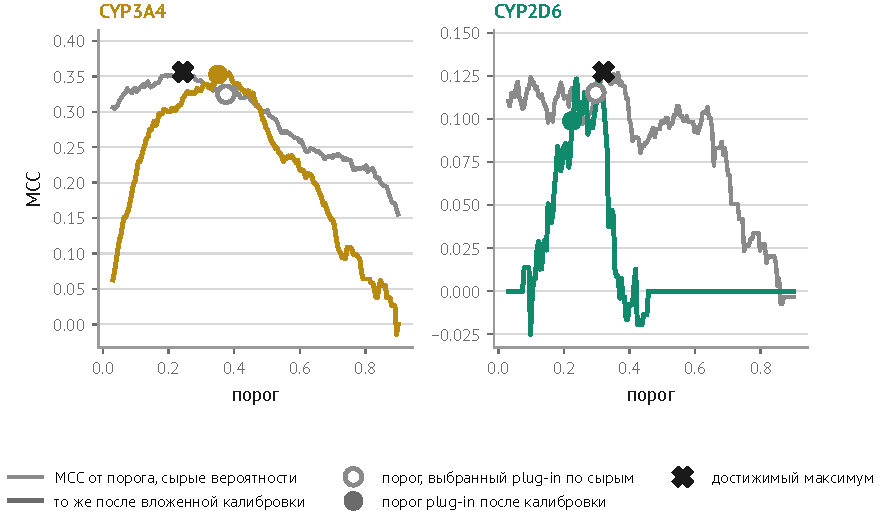
\includegraphics{fig/mcc}
\caption{MCC как функция порога. Слова «при калиброванных $p_i$» оказались не формальностью:
на сырых вероятностях подстановочный порог промахивается мимо максимума. На CYP3A4 он даёт 0.325 при
достижимых 0.356, на CYP2D6 --- 0.115 при 0.127. На 3A4 промах стоит больше половины всего выигрыша
от подбора порога.}
\label{fig:mcc}
\end{figure}

На сохранённых вероятностях бустинга средняя предсказанная вероятность равна 0.256 против настоящей доли
положительных 0.326 на 3A4 и 0.079 против 0.217 на 2D6. Подстановочный метод берёт на 3A4 порог 0.375
и даёт MCC 0.325, тогда как оптимум при 0.258 даёт 0.358 --- потеря 0.033. Вложенная калибровка Платта
возвращает почти всё: потеря падает до 0.003, показатель Брайера с 0.2075 до 0.1853, чистый выигрыш
$+0.028$ MCC. Больше, чем даёт любая перестановка признаков в наших абляциях.

На 2D6 не окупается. Калибровка чинит калибровку (средняя предсказанная с 0.079 до 0.217, Брайер
с 0.199 до 0.169), а MCC не растёт: изотоническая сжимает достижимый максимум с 0.127 до 0.108, Платт
уводит порог не туда. При MCC порядка 0.12 и 260 положительных на обучение калибратора его собственный
шум съедает пользу.

В архитектуру идёт связка «вложенная калибровка, затем подстановочный порог», с абляцией на каждом
эндпойнте отдельно.

Незакрытая дыра: вероятностная версия \eqref{eq:tdirule} с интегрированием по ансамблю не запускалась
ни разу. Все измеренные варианты правила --- детерминированные подстановочные.
